% Options for packages loaded elsewhere
\PassOptionsToPackage{unicode}{hyperref}
\PassOptionsToPackage{hyphens}{url}
\documentclass[
  ignorenonframetext,
  aspectratio=169,
]{beamer}
\newif\ifbibliography
\usepackage{pgfpages}
\setbeamertemplate{caption}[numbered]
\setbeamertemplate{caption label separator}{: }
\setbeamercolor{caption name}{fg=normal text.fg}
\beamertemplatenavigationsymbolsempty
% remove section numbering
\setbeamertemplate{part page}{
  \centering
  \begin{beamercolorbox}[sep=16pt,center]{part title}
    \usebeamerfont{part title}\insertpart\par
  \end{beamercolorbox}
}
\setbeamertemplate{section page}{
  \centering
  \begin{beamercolorbox}[sep=12pt,center]{section title}
    \usebeamerfont{section title}\insertsection\par
  \end{beamercolorbox}
}
\setbeamertemplate{subsection page}{
  \centering
  \begin{beamercolorbox}[sep=8pt,center]{subsection title}
    \usebeamerfont{subsection title}\insertsubsection\par
  \end{beamercolorbox}
}
% Prevent slide breaks in the middle of a paragraph
\widowpenalties 1 10000
\raggedbottom
\AtBeginPart{
  \frame{\partpage}
}
\AtBeginSection{
  \ifbibliography
  \else
    \frame{\sectionpage}
  \fi
}
\AtBeginSubsection{
  \frame{\subsectionpage}
}
\usepackage{iftex}
\ifPDFTeX
  \usepackage[T1]{fontenc}
  \usepackage[utf8]{inputenc}
  \usepackage{textcomp} % provide euro and other symbols
\else % if luatex or xetex
  \usepackage{unicode-math} % this also loads fontspec
  \defaultfontfeatures{Scale=MatchLowercase}
  \defaultfontfeatures[\rmfamily]{Ligatures=TeX,Scale=1}
\fi
\usepackage{lmodern}
\ifPDFTeX\else
  % xetex/luatex font selection
\fi
% Use upquote if available, for straight quotes in verbatim environments
\IfFileExists{upquote.sty}{\usepackage{upquote}}{}
\IfFileExists{microtype.sty}{% use microtype if available
  \usepackage[]{microtype}
  \UseMicrotypeSet[protrusion]{basicmath} % disable protrusion for tt fonts
}{}
\makeatletter
\@ifundefined{KOMAClassName}{% if non-KOMA class
  \IfFileExists{parskip.sty}{%
    \usepackage{parskip}
  }{% else
    \setlength{\parindent}{0pt}
    \setlength{\parskip}{6pt plus 2pt minus 1pt}}
}{% if KOMA class
  \KOMAoptions{parskip=half}}
\makeatother
\usepackage{longtable,booktabs,array}
\usepackage{caption}
\captionsetup[table]{skip=6pt}
\newcounter{none} % for unnumbered tables
\usepackage{calc} % for calculating minipage widths
\usepackage{caption}
% Make caption package work with longtable
\makeatletter
\def\fnum@table{\tablename~\thetable}
\makeatother
\usepackage{graphicx}
\makeatletter
\newsavebox\pandoc@box
\newcommand*\pandocbounded[1]{% scales image to fit in text height/width
  \sbox\pandoc@box{#1}%
  \Gscale@div\@tempa{\textheight}{\dimexpr\ht\pandoc@box+\dp\pandoc@box\relax}%
  \Gscale@div\@tempb{\linewidth}{\wd\pandoc@box}%
  \ifdim\@tempb\p@<\@tempa\p@\let\@tempa\@tempb\fi% select the smaller of both
  \ifdim\@tempa\p@<\p@\scalebox{\@tempa}{\usebox\pandoc@box}%
  \else\usebox{\pandoc@box}%
  \fi%
}
% Set default figure placement to htbp
\def\fps@figure{htbp}
\makeatother
\setlength{\emergencystretch}{3em} % prevent overfull lines
\providecommand{\tightlist}{%
  \setlength{\itemsep}{0pt}\setlength{\parskip}{0pt}}
% Auto-generated by infrastructure/rendering/_pdf_latex_helpers.py::extract_math_font_preamble.
% Minimal header passed to Pandoc via -H so Beamer slides pick up the same math font
% as the combined-PDF path. Adjust the manuscript's preamble.md to change the font globally.
\usepackage{unicode-math}
\setmathfont{latinmodern-math.otf}

% Manuscript macro/package fallbacks (newcommand -> providecommand).
% Core mathematics
\usepackage{amsmath}
\usepackage{amssymb}
% Document layout
% Tables
\usepackage{booktabs}
% Caption styling (booktabs already loaded above). Small caption font with a
% bold label ("Figure 1", "Table 2") gives the math/figure-heavy layout a
% consistent, journal-like caption rhythm without fighting pandoc-crossref —
% pandoc emits standard \caption{}, and caption/captionsetup only restyle it.
% ── Theorem environments ─────────────────────────────────────────────────
% amsthm is loaded above. The FedGVI<->Friston bridge is stated as a small
% number of theorems/definitions/lemmas/propositions/corollaries; sharing one
% counter (definition/lemma/proposition/corollary all step the `theorem`
% counter) gives a single monotone numbering 1, 2, 3, ... across all kinds, so
% authors can reference them as Theorem 1, Definition 2, Corollary 3 without a
% per-kind counter drifting out of order. Plain style for theorem-like results,
% definition style (upright body) for definitions.
% (algorithm2e intentionally not loaded: this manuscript states results as
% numbered amsthm Theorems/Definitions, not algorithm2e pseudocode.)
% Code listings
\usepackage{listings}
% Typography and formatting
% (siunitx intentionally not loaded: no \SI/\num units appear in this manuscript.)
% Cross-references and citations
% (cleveref and titlesec intentionally not loaded: unavailable in this TeX tree
% and not required. Cross-references resolve through pandoc-crossref's own
% \ref-style names — no \cref appears — and section heading styling falls back
% to the pandoc/LaTeX defaults.)
% ── TeX Live Basic-compatible mono font for code listings ────────────
% Latin Modern Mono is bundled with TeX Live Basic and keeps the manuscript
% renderable on minimal TeX installations. Mathematical Unicode coverage is
% provided separately by Latin Modern Math below, so the code font does not
% need a private JuliaMono installation.
%
% Use the TeX font filename rather than the system-family name: the minimal
% TeX Live fontconfig database may not register the OpenType family even though
% kpsewhich can resolve the bundled files.
% Math font for unicode-math: Latin Modern Math (TeX Live) has full BMP
% coverage including U+2223 (\mid), U+226A/226B (\ll/\gg), and the Greek/
% blackboard letters used in equations. Without an explicit \setmathfont,
% unicode-math falls back to lmroman text font which lacks several glyphs
% and emits "Missing character" warnings on every \mid in math mode.

% Slide layout defaults for warning-clean scientific decks.
\usepackage{etoolbox}
\IfFileExists{xurl.sty}{\usepackage{xurl}}{}
\IfFileExists{seqsplit.sty}{\usepackage{seqsplit}}{\newcommand{\seqsplit}[1]{#1}}
\protected\def\breakseq#1{\seqsplit{#1}}
\protected\def\breaktt#1{\begingroup\ttfamily\seqsplit{#1}\endgroup}
\setlength{\emergencystretch}{6em}
\tolerance=5000
\hbadness=10000
\hfuzz=1pt
\setlength{\tabcolsep}{2pt}
\AtBeginEnvironment{longtable}{\tiny\renewcommand{\arraystretch}{0.86}\setlength{\tabcolsep}{1pt}}
\AtBeginEnvironment{tabular}{\tiny\renewcommand{\arraystretch}{0.86}\setlength{\tabcolsep}{1pt}}
\AtBeginEnvironment{equation}{\tiny}
\AtBeginEnvironment{equation*}{\tiny}
\AtBeginEnvironment{align}{\tiny}
\AtBeginEnvironment{align*}{\tiny}
\AtBeginEnvironment{itemize}{\footnotesize}
\AtBeginEnvironment{enumerate}{\footnotesize}
\AtBeginEnvironment{description}{\footnotesize}
\setbeamerfont{caption}{size=\tiny}
\setbeamerfont{caption name}{size=\tiny}
\setbeamerfont{normal text}{size=\small}
\setbeamerfont{frametitle}{size=\small}
\setbeamerfont{section title}{size=\footnotesize}
\setbeamerfont{subsection title}{size=\footnotesize}
\setbeamertemplate{section page}{%
  \centering
  \begin{beamercolorbox}[sep=12pt,center,wd=\paperwidth]{section title}
    \parbox{0.86\paperwidth}{\centering\usebeamerfont{section title}\insertsection\par}
  \end{beamercolorbox}
}
\setbeamertemplate{subsection page}{%
  \centering
  \begin{beamercolorbox}[sep=8pt,center,wd=\paperwidth]{subsection title}
    \parbox{0.86\paperwidth}{\centering\usebeamerfont{subsection title}\insertsubsection\par}
  \end{beamercolorbox}
}
\setlength{\abovecaptionskip}{2pt}
\setlength{\belowcaptionskip}{0pt}

% Natbib and cross-reference fallbacks — slides don't load natbib
% or cleveref, but combined-PDF manuscript prose may emit these
% commands. The fallback renders citations as a bracketed key list
% and cross-references as detokenized labels so slides don't fail on
% undefined control sequences or raw underscores. \providecommand is
% a no-op if packages load later.
\providecommand{\citep}[1]{[#1]}
\providecommand{\citet}[1]{#1}
\providecommand{\citealp}[1]{#1}
\providecommand{\citeauthor}[1]{#1}
\providecommand{\citeyear}[1]{#1}
\providecommand{\cref}[1]{\texttt{\detokenize{#1}}}
\providecommand{\Cref}[1]{\texttt{\detokenize{#1}}}
\providecommand{\crefrange}[2]{\texttt{\detokenize{#1}}--\texttt{\detokenize{#2}}}
\providecommand{\Crefrange}[2]{\texttt{\detokenize{#1}}--\texttt{\detokenize{#2}}}
\providecommand{\paragraph}[1]{\textbf{#1}\ }

% Opt-in accessible presentation profile.
\setbeamerfont{normal text}{size*={20pt}{24pt}}
\setbeamerfont{frametitle}{size*={28pt}{32pt}}
\setbeamerfont{section title}{size*={28pt}{32pt}}
\setbeamerfont{subsection title}{size*={28pt}{32pt}}
\setbeamerfont{caption}{size*={16pt}{19pt}}
\setbeamerfont{caption name}{size*={16pt}{19pt}}
\setbeamerfont{itemize/enumerate body}{size*={20pt}{24pt}}
\setbeamerfont{itemize/enumerate subbody}{size*={20pt}{24pt}}
\setbeamerfont{itemize/enumerate subsubbody}{size*={20pt}{24pt}}
\setbeamerfont{itemize item}{size*={20pt}{24pt}}
\setbeamerfont{itemize subitem}{size*={20pt}{24pt}}
\setbeamerfont{itemize subsubitem}{size*={20pt}{24pt}}
\setbeamerfont{description body}{size*={20pt}{24pt}}
\setbeamerfont{description item}{size*={20pt}{24pt}}
\setbeamerfont{quote}{size*={20pt}{24pt}}
\setbeamerfont{quotation}{size*={20pt}{24pt}}
\AtBeginEnvironment{longtable}{\fontsize{20pt}{24pt}\selectfont}
\AtBeginEnvironment{tabular}{\fontsize{20pt}{24pt}\selectfont}
\AtBeginEnvironment{equation}{\fontsize{20pt}{24pt}\selectfont}
\AtBeginEnvironment{equation*}{\fontsize{20pt}{24pt}\selectfont}
\AtBeginEnvironment{align}{\fontsize{20pt}{24pt}\selectfont}
\AtBeginEnvironment{align*}{\fontsize{20pt}{24pt}\selectfont}
\AtBeginEnvironment{itemize}{\fontsize{20pt}{24pt}\selectfont}
\AtBeginEnvironment{enumerate}{\fontsize{20pt}{24pt}\selectfont}
\AtBeginEnvironment{description}{\fontsize{20pt}{24pt}\selectfont}
\AtBeginDocument{\usebeamerfont{normal text}}
\newlength{\AFSlideTableWidth}
% The fixed footer reservation is calibrated with the semantic seven-line regular-body budget.
\setbeamertemplate{footline}{%
  \leavevmode\vbox{%
    \hbox{%
      \begin{beamercolorbox}[wd=\paperwidth,ht=16pt,dp=3pt,center]{author in head/foot}%
        \fontsize{16pt}{19pt}\selectfont Untagged PDF derivative \textbar\ \href{../web/index.html}{HTML reader}%
      \end{beamercolorbox}%
    }%
    \vskip6pt%
  }%
}
% Accessible footer reserved height: 25pt.

\newtheorem{proposition}{Proposition}
\newtheorem{hypothesis}{Hypothesis}
\newtheorem{remark}[theorem]{Remark}
\newtheorem{axiom}{Axiom}
\newtheorem{property}{Property}
\usepackage{bookmark}
\IfFileExists{xurl.sty}{\usepackage{xurl}}{} % add URL line breaks if available
\urlstyle{same}
% fallback for those not using the hyperref driver hyperxmp:
\makeatletter
\@ifundefined{xmpquote}{\newcommand{\xmpquote}[1]{#1}}{}
\makeatother
\hypersetup{
  hidelinks,
  pdfcreator={LaTeX via pandoc}}

\author{\texorpdfstring{}{}}
\date{}

\begin{document}

\begin{frame}{Configured BMR sign control passed}
\protect\phantomsection\label{sec:results-emergence}
The first two studies fixed the model structure. This third study
instead checks the sign of a configured Bayesian-model-reduction
comparison. Its estimand is the BMR free-energy difference for two
candidate likelihood-column prunings.
\end{frame}

\begin{frame}{Configured BMR sign\ldots{} (part 2)}
The categorical diagnostic is related to the model-reduction mechanism
discussed by Friston et al. (Friston et al. 2024) and the post-hoc BMR
lineage (Friston and Penny 2011). It is not a discovery claim about
structure emergence.
\end{frame}

\begin{frame}{Configured BMR sign\ldots{} (part 3)}
The fixed posterior ranges over \(n = 4\) candidate states. One
likelihood column is unsupported by the configured evidence; another is
a supported control. BMR substitutes a reduced prior for each candidate
and computes \(\Delta F\) eq.~20. This is one
deterministic closed-form comparison,
\end{frame}

\begin{frame}{Configured BMR sign\ldots{} (part 4)}
so no resampled sample, confidence interval, or paired test applies
(Smith et al. 2022).
\end{frame}

\begin{frame}{Configured BMR sign\ldots{} (part 5)}
\(\Delta F\) is positive for the declared redundant-column pruning, so
the reduced candidate is favored for this fixed posterior.
\textbf{Redundant-column result:} \(\Delta F=3.68\); the configured
reduction is accepted.
\end{frame}

\begin{frame}{Configured BMR sign\ldots{} (part 6)}
It is negative for the declared supported-column control.
\textbf{Supported-column control:} \(\Delta F=-27.67\); that reduction
is rejected.

\textbf{Configured sign-control disposition:} redundant accepted and
supported rejected, recorded as Yes.
\end{frame}

\begin{frame}{Configured BMR sign\ldots{} (part 7)}
The observed sign pattern
\(\Delta F_{\text{redundant}} > 0 > \Delta F_{\text{supported}}\) passes
the configured control: this fixed posterior favors pruning the declared
redundant column and rejects pruning the declared supported column.
\end{frame}

\begin{frame}{Configured BMR sign\ldots{} (part 8)}
It does not show that arbitrary data or model families will discover,
prune, or retain the correct structure.
\end{frame}

\begin{frame}{Configured BMR sign\ldots{} (part 9)}
\begin{figure}
\centering
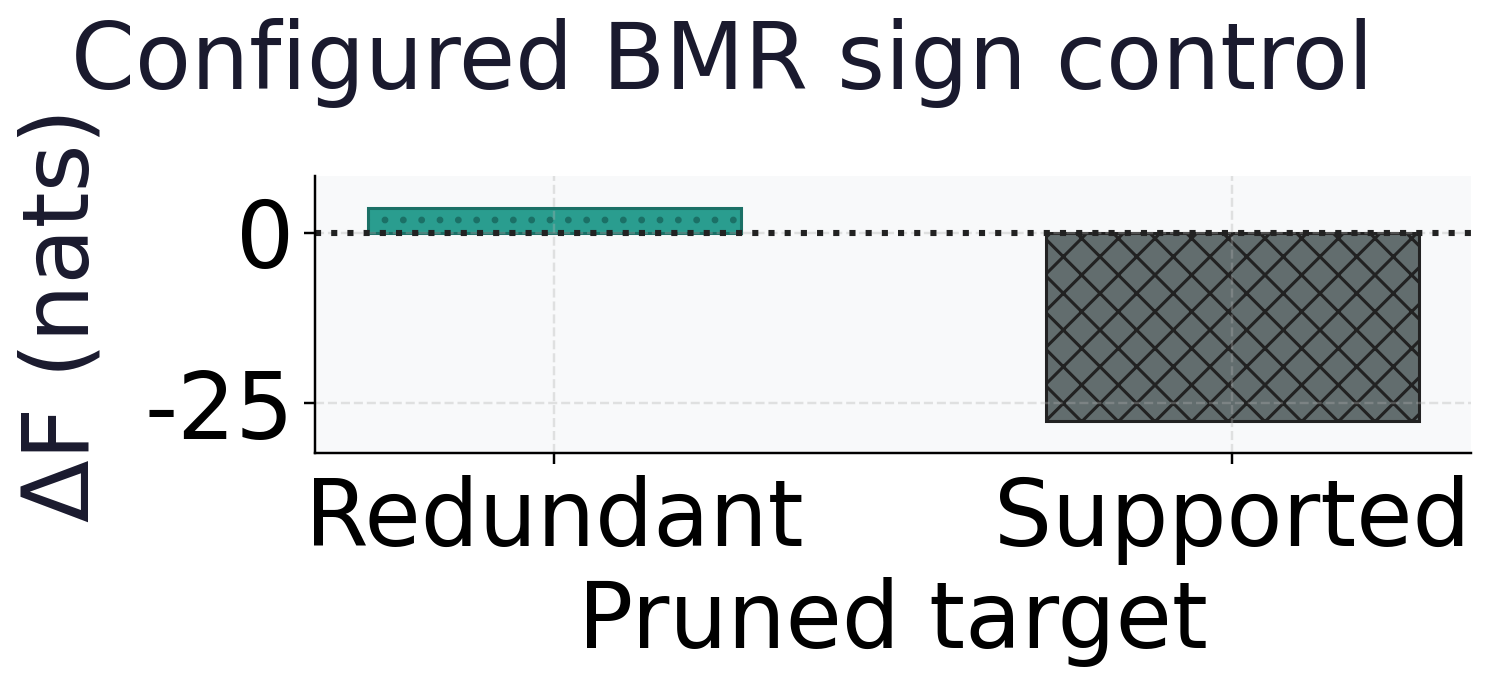
\includegraphics[keepaspectratio,width=0.98\linewidth,height=0.8\textheight,alt={Both signed model-reduction gains on one nats scale; hatches distinguish targets and a dotted rule marks zero.}]{../figures/emergence_bmr.slide-controls.png}
\refstepcounter{figure}\label{fig:emergence-bmr-slide-panel-1}
\end{figure}
\end{frame}

\begin{frame}{Configured BMR sign\ldots{} (part 10)}
\begin{figure}
\centering
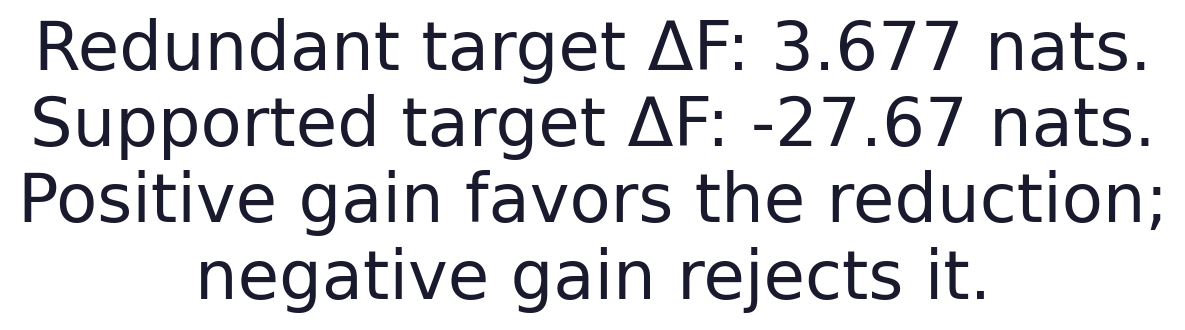
\includegraphics[keepaspectratio,width=0.98\linewidth,height=0.8\textheight,alt={Redundant target ΔF: 3.677 nats. Supported target ΔF: -27.67 nats. Positive gain favors the reduction; negative gain rejects it.}]{../figures/emergence_bmr.slide-values.png}
\refstepcounter{figure}\label{fig:emergence-bmr-slide-panel-2}
\end{figure}
\end{frame}

\begin{frame}{Configured BMR sign\ldots{} (part 11)}
\begin{figure}
\centering
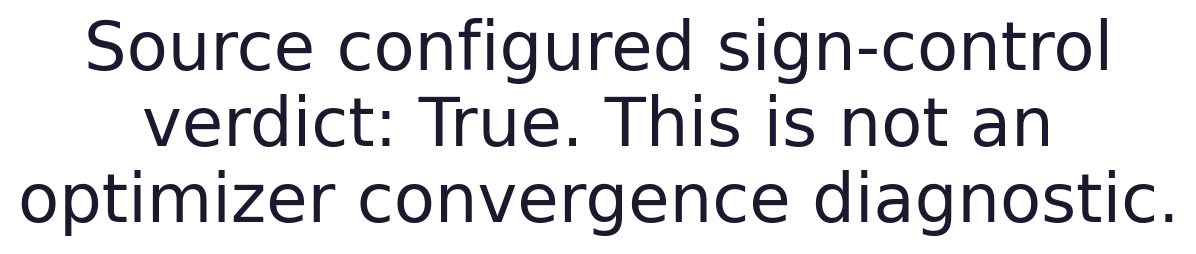
\includegraphics[keepaspectratio,width=0.98\linewidth,height=0.8\textheight,alt={Source configured sign-control verdict: True. This is not an optimizer convergence diagnostic.}]{../figures/emergence_bmr.slide-verdict.png}
\refstepcounter{figure}\label{fig:emergence-bmr-slide-panel-3}
\end{figure}
\end{frame}

\begin{frame}{Configured BMR sign\ldots{} (part 12)}
\begin{figure}
\centering
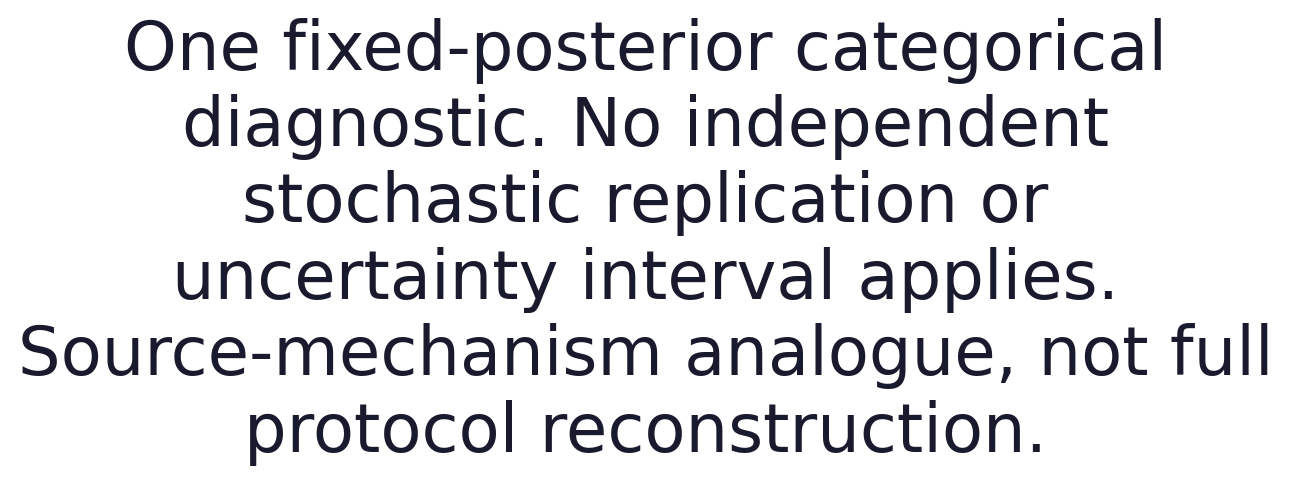
\includegraphics[keepaspectratio,width=0.98\linewidth,height=0.8\textheight,alt={One fixed-posterior categorical diagnostic. No independent stochastic replication or uncertainty interval applies. Source-mechanism analogue, not full protocol reconstruction.}]{../figures/emergence_bmr.slide-scope.png}
\refstepcounter{figure}\label{fig:emergence-bmr-slide-panel-4}
\end{figure}
\end{frame}

\begin{frame}{Configured BMR sign\ldots{} (part 13)}
fig.~12 contrasts the two configured prunings and
reports the sign control.
\end{frame}

\begin{frame}{Configured BMR sign\ldots{} (part 14)}
Studies 1--3 all ran in a \emph{trusting} world, where every broadcast
belief is honest. The contamination sweep that follows removes that
assumption, and it is the point at which the three robustness axes of
sec.~7.2.1 begin to diverge.
\end{frame}

\end{document}
